% ------------------------------------------------
% RESULTADOS
% ------------------------------------------------

\chapter{Resultados}

\section{Introducción}
La evaluación experimental de Praeco se ha realizado de forma progresiva durante las distintas etapas de desarrollo. Los primeros ensayos permitieron caracterizar el comportamiento del OCR y detectar limitaciones del corrector inicial. Posteriormente se incorporaron reglas de protección, vocabulario adaptativo y un mecanismo de aprendizaje incremental. Finalmente, se estableció una metodología que separa de forma explícita los experimentos realizados con aprendizaje activo de aquellos ejecutados con los recursos lingüísticos congelados.

Esta separación es necesaria para interpretar correctamente los resultados. La variable \texttt{modo\_aprendizaje}, almacenada en cada experimento, identifica las dos condiciones de funcionamiento:

\begin{itemize}[noitemsep]
	\item \textbf{\texttt{modo\_aprendizaje = true}:} Praeco se encuentra en fase de desarrollo y aprendizaje. El \textit{ground truth} puede utilizarse para registrar errores recurrentes del OCR y actualizar los recursos adaptativos cuando se cumplen los criterios establecidos.
	\item \textbf{\texttt{modo\_aprendizaje = false}:} Praeco utiliza los recursos lingüísticos disponibles, pero no los modifica. Esta configuración se emplea para la validación con el conocimiento congelado, evitando que las muestras evaluadas alteren simultáneamente el comportamiento del corrector.
\end{itemize}

Por tanto, los resultados obtenidos en ambas modalidades no deben mezclarse como si pertenecieran a una única condición experimental. Los ensayos con aprendizaje activo permiten estudiar la construcción del conocimiento adaptativo, mientras que los realizados con aprendizaje desactivado permiten evaluar el comportamiento del sistema con una configuración fija.

La versión final del trabajo utiliza además Praeco Análisis como aplicación independiente para procesar los experimentos generados por Praeco Desarrollo y estudiar CER, WER, tiempos, variables de calidad y diferencias entre las dos modalidades de aprendizaje.

% ------------------------------------------------
\section{Métricas de evaluación}
% ------------------------------------------------

\subsection{Character Error Rate (CER)}
La métrica CER (\textit{Character Error Rate}) cuantifica el error a nivel de caracteres respecto al texto real o \textit{ground truth}. Se calcula mediante:

\begin{equation}
	\mathrm{CER}=\frac{S+D+I}{N}
\end{equation}

donde $S$ es el número de sustituciones, $D$ el número de eliminaciones, $I$ el número de inserciones y $N$ el número de caracteres del texto de referencia. El cálculo se basa en la distancia de Levenshtein. Un valor de CER igual a cero representa una coincidencia perfecta.

\subsection{Word Error Rate (WER)}
La métrica WER (\textit{Word Error Rate}) aplica el mismo principio a nivel de palabras:

\begin{equation}
	\mathrm{WER}=\frac{S+D+I}{N}
\end{equation}

donde, en este caso, $S$, $D$ e $I$ representan sustituciones, eliminaciones e inserciones de palabras y $N$ es el número de palabras del texto de referencia. CER y WER se calculan tanto para la salida OCR de referencia como para el texto obtenido después de aplicar el corrector de Praeco.

\subsection{Criterio de comparación}
Para cuantificar el efecto del corrector se utilizan las diferencias:

\begin{equation}
	\Delta\mathrm{CER}=\mathrm{CER}_{\mathrm{CORR}}-\mathrm{CER}_{\mathrm{OCR}}
\end{equation}

\begin{equation}
	\Delta\mathrm{WER}=\mathrm{WER}_{\mathrm{CORR}}-\mathrm{WER}_{\mathrm{OCR}}
\end{equation}

Un valor negativo indica una reducción del error, un valor igual a cero indica que la corrección no ha modificado la métrica y un valor positivo indica un empeoramiento. Este criterio permite incluir también los casos en los que el OCR original presenta error cero; estos experimentos son especialmente relevantes para detectar si el corrector modifica de forma incorrecta un texto que ya era correcto.

\begin{figure}[htbp]
	\centering
	
	\resizebox{0.96\textwidth}{!}{%
		\begin{tikzpicture}[
			x=1cm,
			y=1cm,
			box/.style={
				draw,
				rounded corners,
				align=center,
				minimum width=5.2cm,
				minimum height=0.80cm,
				inner sep=5pt,
				font=\small
			},
			modebox/.style={
				draw,
				rounded corners,
				align=center,
				minimum width=5.5cm,
				minimum height=0.95cm,
				inner sep=5pt,
				font=\small
			},
			decision/.style={
				draw,
				diamond,
				aspect=2.3,
				align=center,
				minimum width=3.2cm,
				minimum height=1.0cm,
				inner sep=2pt,
				font=\small
			},
			resultbox/.style={
				draw,
				rounded corners,
				align=center,
				minimum width=3.6cm,
				minimum height=1.05cm,
				inner sep=4pt,
				font=\small
			},
			line/.style={
				-{Latex[length=1.8mm]},
				thick
			}
			]
			\node[box] (inicio) at (0,0)
			{\textbf{Inicio de la evaluación}};
			
			\node[box] (recursos) at (0,-1.5)
			{Carga de recursos\\
				diccionarios y configuración};
			
			\node[box] (modo) at (0,-3.0)
			{Selección del modo de ejecución\\
				\texttt{modoAprendizajePraeco}};
			
			\node[decision] (decision) at (0,-5.0)
			{¿Aprendizaje\\activo?};
			\node[modebox] (aprendizaje) at (-5.0,-7.0)
			{\textbf{FASE DE APRENDIZAJE}\\
				\texttt{modoAprendizajePraeco = true}};
			
			\node[box] (procA) at (-5.0,-8.7)
			{Procesamiento de la imagen\\
				captura $\rightarrow$ calidad $\rightarrow$ OCR};
			
			\node[box] (corrA) at (-5.0,-10.3)
			{Corrección y comparación\\
				con el \textit{ground truth}};
			
			\node[box] (errorA) at (-5.0,-11.9)
			{Registro de asociaciones\\
				en \texttt{errores\_ocr.json}};
			
			\node[box] (dicA) at (-5.0,-13.6)
			{Actualización de\\
				\texttt{diccionario\_adaptativo.json}\\
				según frecuencia y conflictos};
			
			\node[box] (csvA) at (-5.0,-15.4)
			{Registro del experimento\\
				en \texttt{experimentos.csv}};
			\node[modebox] (validacion) at (5.0,-7.0)
			{\textbf{FASE DE VALIDACIÓN}\\
				\texttt{modoAprendizajePraeco = false}};
			
			\node[box] (procV) at (5.0,-8.7)
			{Procesamiento de la imagen\\
				captura $\rightarrow$ calidad $\rightarrow$ OCR};
			
			\node[box] (corrV) at (5.0,-10.3)
			{Corrección utilizando\\
				recursos congelados};
			
			\node[box] (gtV) at (5.0,-11.9)
			{Comparación con el\\
				\textit{ground truth} auditado};
			
			\node[box] (noaprende) at (5.0,-13.6)
			{Sin actualización de\\
				los recursos de aprendizaje};
			
			\node[box] (csvV) at (5.0,-15.4)
			{Registro del experimento\\
				en \texttt{experimentos.csv}};
			\draw[line] (inicio) -- (recursos);
			\draw[line] (recursos) -- (modo);
			\draw[line] (modo) -- (decision);
			
			% Rama TRUE
			\draw[line]
			(decision.west)
			-- ++(-1.2,0)
			|- node[pos=0.25, above, font=\scriptsize]
			{\texttt{true}}
			(aprendizaje.north);
			
			% Rama FALSE
			\draw[line]
			(decision.east)
			-- ++(1.2,0)
			|- node[pos=0.25, above, font=\scriptsize]
			{\texttt{false}}
			(validacion.north);
			\draw[line] (aprendizaje) -- (procA);
			\draw[line] (procA) -- (corrA);
			\draw[line] (corrA) -- (errorA);
			\draw[line] (errorA) -- (dicA);
			\draw[line] (dicA) -- (csvA);
			\draw[line] (validacion) -- (procV);
			\draw[line] (procV) -- (corrV);
			\draw[line] (corrV) -- (gtV);
			\draw[line] (gtV) -- (noaprende);
			\draw[line] (noaprende) -- (csvV);
			% Punto central de convergencia
			\coordinate (union) at (0,-17.0);
			
			\draw[line]
			(csvA.south)
			-- ++(0,-0.7)
			-| (union);
			
			\draw[line]
			(csvV.south)
			-- ++(0,-0.7)
			-| (union);
			
			\node[
			box,
			minimum width=7.0cm,
			minimum height=1.1cm
			] (analisis) at (0,-18.4)
			{\textbf{PRAECO ANÁLISIS}\\
				Lectura y procesamiento de \texttt{experimentos.csv}};
			
			\draw[line] (union) -- (analisis);
			\node[resultbox] (cer) at (-8.0,-21.0)
			{\textbf{CER y WER}\\
				OCR original\\
				y corregido};
			
			\node[resultbox] (estadistica) at (-4.0,-21.0)
			{\textbf{Estadísticos}\\
				media\\
				desviación típica};
			
			\node[resultbox] (variacion) at (0,-21.0)
			{\textbf{Variación}\\
				$\Delta$CER\\
				$\Delta$WER};
			
			\node[resultbox] (clasificacion) at (4.0,-21.0)
			{\textbf{Clasificación}\\
				mejora, empeora\\
				o sin cambio};
			
			\node[resultbox] (tiempos) at (8.0,-21.0)
			{\textbf{Tiempos}\\
				captura, OCR,\\
				corrección y alérgenos};
			% Línea horizontal de distribución
			\coordinate (distribucion) at (0,-19.8);
			
			\draw[thick] (analisis.south) -- (distribucion);
			
			\draw[thick] (-8.0,-19.8) -- (8.0,-19.8);
			
			\draw[line] (-8.0,-19.8) -- (cer.north);
			\draw[line] (-4.0,-19.8) -- (estadistica.north);
			\draw[line] (0,-19.8) -- (variacion.north);
			\draw[line] (4.0,-19.8) -- (clasificacion.north);
			\draw[line] (8.0,-19.8) -- (tiempos.north);
			\node[
			box,
			minimum width=8.0cm,
			minimum height=1.1cm
			] (resultado) at (0,-23.6)
			{\textbf{RESULTADOS Y CONCLUSIONES}\\
				Evaluación del efecto del corrector y del aprendizaje};
			\coordinate (unionFinal) at (0,-22.4);
			
			\draw[thick] (cer.south) -- ++(0,-0.5) -| (unionFinal);
			\draw[thick] (estadistica.south) -- ++(0,-0.5) -| (unionFinal);
			\draw[thick] (variacion.south) -- (unionFinal);
			\draw[thick] (clasificacion.south) -- ++(0,-0.5) -| (unionFinal);
			\draw[thick] (tiempos.south) -- ++(0,-0.5) -| (unionFinal);
			
			\draw[line] (unionFinal) -- (resultado.north);
			
		\end{tikzpicture}%
	}
	
	\caption{Flujo de evaluación experimental de Praeco.}
	
	\label{fig:flujo-evaluacion-praeco}
	
\end{figure}

\newpage

Los experimentos con aprendizaje activo permiten actualizar los recursos adaptativos, mientras que la validación se realiza con dichos recursos congelados. Los resultados registrados son posteriormente procesados mediante Praeco Análisis.

% ------------------------------------------------
\section{Resultados preliminares}
% ------------------------------------------------

En una primera etapa se realizaron cinco experimentos con etiquetas reales de productos alimentarios. Estos resultados corresponden a una versión anterior del corrector y se mantienen en la memoria porque fueron determinantes para identificar los problemas que posteriormente motivaron la incorporación de reglas de protección y aprendizaje adaptativo.

\begin{table}[htbp]
	\centering
	\caption{Resultados de los cinco experimentos preliminares.}
	\label{tab:resultados-preliminares}
	\vspace{0.2cm}
	\begin{tabular}{ccccc}
		\toprule
		\textbf{Exp.} & \textbf{CER OCR} & \textbf{CER Corr.} & \textbf{WER OCR} & \textbf{WER Corr.} \\
		\midrule
		1 & 0.1969 & 0.2073 & 0.2778 & 0.3333 \\
		2 & 0.1265 & 0.1344 & 0.2162 & 0.2432 \\
		3 & 0.0941 & 0.0941 & 0.2895 & 0.2632 \\
		4 & 0.0407 & 0.0407 & 0.2174 & 0.2174 \\
		5 & 0.1165 & 0.1225 & 0.1829 & 0.2195 \\
		\bottomrule
	\end{tabular}
\end{table}

Los valores medios fueron:

\begin{equation}
	\overline{\mathrm{CER}}_{\mathrm{OCR}}=0.1149,
	\qquad
	\overline{\mathrm{CER}}_{\mathrm{CORR}}=0.1198
\end{equation}

\begin{equation}
	\overline{\mathrm{WER}}_{\mathrm{OCR}}=0.2368,
	\qquad
	\overline{\mathrm{WER}}_{\mathrm{CORR}}=0.2553
\end{equation}

Por tanto, en esta primera versión el corrector no produjo una mejora global. Sin embargo, el análisis individual mostró comportamientos diferentes. En el experimento 3, por ejemplo, el WER disminuyó de 0.2895 a 0.2632, mientras que en otros experimentos aparecieron sustituciones incorrectas que incrementaron el error.

Estos resultados fueron útiles para orientar el desarrollo hacia un corrector más conservador: si una sustitución no presenta suficiente confianza, es preferible conservar el término reconocido por el OCR antes que introducir una modificación potencialmente errónea.

% ------------------------------------------------
\section{Evolución del corrector}
% ------------------------------------------------

A partir de los resultados preliminares se incorporaron mecanismos destinados a reducir las correcciones espurias. Entre ellos se encuentran la protección de números y unidades, palabras cortas, \textit{stopwords}, términos presentes en los diccionarios, determinados nombres propios y vocabulario específico del dominio alimentario.

También se implementó un sistema de aprendizaje incremental. Durante la fase de aprendizaje, Praeco compara el OCR con el \textit{ground truth}, registra asociaciones plausibles en \texttt{errores\_ocr.json}, incrementa su frecuencia cuando vuelven a aparecer y controla posibles conflictos. Cuando se cumplen los criterios definidos, el término correcto puede incorporarse como vocabulario válido a \texttt{diccionario\_adaptativo.json}.

El diccionario adaptativo no debe interpretarse como una tabla destinada a convertir cualquier término desconocido en la palabra española más próxima. Su función es almacenar vocabulario válido aprendido durante el desarrollo. Este comportamiento es especialmente importante en etiquetas multilingües. Por ejemplo, \textit{bianco} puede aparecer legítimamente en una etiqueta italiana; si el término forma parte del texto real, debe conservarse y no sustituirse por \textit{blanco}.

% ------------------------------------------------
\section{Ensayos con aprendizaje activo}
% ------------------------------------------------

Los experimentos ejecutados con:

\begin{center}
	\texttt{modoAprendizajePraeco = true}
\end{center}

corresponden a la fase de desarrollo y aprendizaje. En esta modalidad, Praeco puede utilizar el \textit{ground truth} para actualizar sus recursos adaptativos después de guardar la evaluación.

En uno de los conjuntos de pruebas realizados durante la evolución de Praeco se analizaron cuatro capturas y se obtuvo una reducción del CER medio desde aproximadamente 0.03086 hasta 0.02587. Para WER, el valor medio pasó aproximadamente de 0.07563 a 0.04404. Expresado como reducción relativa del error, estos cambios corresponden aproximadamente a un 16.19\% para CER y un 41.77\% para WER.

\begin{table}[htbp]
	\centering
	\caption{Resumen de un ensayo con aprendizaje activo.}
	\label{tab:aprendizaje-activo}
	\vspace{0.2cm}
	\begin{tabular}{lccc}
		\toprule
		\textbf{Métrica} & \textbf{OCR} & \textbf{Corregido} & \textbf{Reducción relativa} \\
		\midrule
		CER & 0.03086 & 0.02587 & 16.19\% \\
		WER & 0.07563 & 0.04404 & 41.77\% \\
		\bottomrule
	\end{tabular}
\end{table}

En ese conjunto se identificaron tres correcciones efectuadas por Praeco y las tres resultaron correctas. El resultado muestra que el conocimiento adaptativo puede ser útil cuando las asociaciones aprendidas representan adecuadamente los errores encontrados.

No obstante, estos valores no deben interpretarse como una validación independiente de la capacidad de generalización. El aprendizaje se encuentra habilitado y el objetivo de esta fase es construir y depurar el conocimiento que posteriormente será congelado para la evaluación.

% ------------------------------------------------
\section{Validación con aprendizaje desactivado}
% ------------------------------------------------

Para separar el aprendizaje de la evaluación se realizaron posteriormente ensayos con:

\begin{center}
	\texttt{modoAprendizajePraeco = false}
\end{center}

En esta configuración, Praeco carga los recursos lingüísticos disponibles, pero no modifica \texttt{errores\_ocr.json} ni \texttt{diccionario\_adaptativo.json} a partir de las muestras evaluadas. De esta forma, el corpus de validación no altera simultáneamente el conocimiento utilizado por el corrector.

Durante esta etapa se construyó un corpus de 28 capturas correspondientes a diferentes productos. El procedimiento experimental incluyó la revisión de las imágenes originales y la auditoría manual del \textit{ground truth}. Esta revisión es necesaria porque una transcripción de referencia incorrecta puede atribuir al OCR o al corrector un error que realmente no existe.

En una evaluación intermedia, correspondiente a 21 muestras cuyo \textit{ground truth} ya había sido auditado en ese momento, se obtuvieron los siguientes valores medios:

\begin{equation}
	\overline{\mathrm{CER}}_{\mathrm{OCR}}=0.05909,
	\qquad
	\overline{\mathrm{CER}}_{\mathrm{CORR}}=0.05981
\end{equation}

\begin{equation}
	\overline{\mathrm{WER}}_{\mathrm{OCR}}=0.19732,
	\qquad
	\overline{\mathrm{WER}}_{\mathrm{CORR}}=0.20131
\end{equation}

La variación relativa fue aproximadamente de $+1.21\%$ para CER y $+2.02\%$ para WER. En consecuencia, en este subconjunto de validación congelada el corrector no produjo una mejora global, aunque la diferencia respecto al OCR original fue reducida.

\begin{table}[htbp]
	\centering
	\caption{Evaluación intermedia con aprendizaje desactivado y \textit{ground truth} auditado.}
	\label{tab:validacion-congelada}
	\vspace{0.2cm}
	\begin{tabular}{lccc}
		\toprule
		\textbf{Métrica} & \textbf{OCR} & \textbf{Corregido} & \textbf{Variación relativa} \\
		\midrule
		CER & 0.05909 & 0.05981 & +1.21\% \\
		WER & 0.19732 & 0.20131 & +2.02\% \\
		\bottomrule
	\end{tabular}
\end{table}

Es importante señalar que estos valores corresponden al análisis intermedio de 21 muestras auditadas y no deben confundirse con el corpus de 28 capturas utilizado en una etapa posterior de auditoría. Ambas evaluaciones forman parte de etapas intermedias del desarrollo. Tras completar la depuración del \textit{ground truth} y ampliar el conjunto experimental, se realizó la validación final con los recursos de aprendizaje congelados. El conjunto utilizado para los resultados globales finales de este trabajo está formado por 63 registros, todos ellos obtenidos con \texttt{modo\_aprendizaje = false}. Salvo que se indique expresamente lo contrario, las métricas globales presentadas en la parte final de este capítulo corresponden a esos 63 registros.

Los ensayos con aprendizaje desactivado permitieron además localizar falsos positivos concretos del corrector y comprobar la necesidad de proteger vocabulario legítimo que puede no pertenecer al castellano. En estos casos, el criterio de referencia es siempre el texto realmente impreso en la etiqueta y no la proximidad de la palabra a un término español.

% ------------------------------------------------
\section{Importancia de la auditoría del \textit{ground truth}}
% ------------------------------------------------

La validación puso de manifiesto que la calidad del \textit{ground truth} condiciona directamente CER y WER. Una referencia incorrecta puede hacer que una lectura correcta del OCR se contabilice como error o que una modificación incorrecta del corrector parezca una mejora.

Por este motivo, la metodología final incorpora una auditoría manual del texto real mediante comparación directa con las imágenes originales. Esta precaución es especialmente relevante en etiquetas multilingües, nombres propios, marcas, abreviaturas, cantidades y expresiones poco frecuentes. La presencia de una palabra italiana, inglesa o francesa no constituye por sí misma un error del OCR si esa palabra aparece realmente en la etiqueta.

% ------------------------------------------------
\section{Interpretación conjunta de los modos de aprendizaje}
% ------------------------------------------------

Los dos valores de \texttt{modo\_aprendizaje} representan objetivos experimentales distintos:

\begin{itemize}
	\item Con \texttt{modo\_aprendizaje = true}, el objetivo es \textbf{aprender y depurar}. El sistema puede utilizar el \textit{ground truth} para registrar errores y ampliar de forma controlada el vocabulario adaptativo.
	\item Con \texttt{modo\_aprendizaje = false}, el objetivo es \textbf{validar}. Los recursos permanecen congelados y las muestras de validación no pueden modificar el conocimiento utilizado durante la propia prueba.
\end{itemize}

Por ello, una mejora observada con aprendizaje activo demuestra que el sistema puede aprovechar conocimiento adaptativo, pero no constituye por sí sola una medida independiente de generalización. La validación con aprendizaje desactivado proporciona una evaluación metodológicamente más adecuada del comportamiento del corrector una vez fijados sus recursos.

La secuencia metodológica adoptada para la evaluación final puede resumirse como:

\begin{center}
	\textbf{aprendizaje} $\rightarrow$ \textbf{auditoría} $\rightarrow$ \textbf{congelación de recursos} $\rightarrow$ \textbf{validación}
\end{center}

% ------------------------------------------------
\section{Análisis de las causas de error}
% ------------------------------------------------

El análisis individual de los experimentos permitió identificar diferentes fuentes de error:

\begin{itemize}[noitemsep]
	\item errores generados por el OCR debido a desenfoque, iluminación, contraste, tamaño de los caracteres o características tipográficas de la etiqueta;
	\item palabras válidas no presentes inicialmente en los recursos lingüísticos;
	\item términos pertenecientes a otros idiomas que forman parte legítima del etiquetado;
	\item palabras cortas, para las que una pequeña distancia de edición puede producir candidatos incorrectos;
	\item códigos, cantidades, unidades y expresiones alfanuméricas que no deben tratarse como palabras ordinarias;
	\item correcciones ambiguas en las que varios candidatos presentan puntuaciones similares;
	\item errores severos del OCR para los que no existe un candidato suficientemente próximo y fiable.
\end{itemize}

Estos resultados justifican la estrategia conservadora adoptada: ante una corrección insuficientemente fiable, resulta preferible conservar el término reconocido por el OCR antes que introducir una sustitución potencialmente incorrecta.

% ------------------------------------------------
\section{Análisis temporal}
% ------------------------------------------------

Además de CER y WER, Praeco registra el tiempo empleado en las principales etapas del procesamiento. Entre las variables almacenadas se encuentran \texttt{t\_captura}, \texttt{t\_ocr}, \texttt{t\_correccion} y \texttt{t\_alergenos}. Estas medidas permiten estudiar el coste computacional de cada etapa y comprobar si la incorporación del corrector y del detector de alérgenos mantiene un comportamiento compatible con el uso interactivo de la aplicación.

El análisis temporal debe interpretarse de forma independiente de CER y WER: los tiempos describen el coste de procesamiento, mientras que CER y WER cuantifican la precisión textual. Praeco Análisis permite estudiar conjuntamente ambas dimensiones sin introducir lógica estadística adicional en la aplicación destinada al usuario final.

\begin{table}[htbp]
	\centering
	\caption{Tiempos medios de procesamiento por producto durante la fase de validación.}
	\label{tab:tiempos-productos}
	\renewcommand{\arraystretch}{1.20}
	\setlength{\tabcolsep}{5pt}
	
	\begin{tabular}{lrrrrr}
		\toprule
		\textbf{Producto} &
		\textbf{Captura} &
		\textbf{OCR} &
		\textbf{Corrección} &
		\textbf{Alérgenos} &
		\textbf{Total} \\
		& \textbf{(ms)} & \textbf{(ms)} & \textbf{(ms)}
		& \textbf{(ms)} & \textbf{(ms)} \\
		\midrule
		
		Fairy          & 4060.3 & 226.3 & 71.3  & 6.3  & 4364.3 \\
		KH-7           & 3944.8 & 199.0 & 48.5  & 5.5  & 4197.8 \\
		Gallina Blanca & 3984.0 & 215.7 & 59.7  & 6.0  & 4265.3 \\
		Eroski         & 4044.7 & 271.3 & 121.3 & 17.7 & 4455.0 \\
		Azucarera      & 4229.3 & 333.7 & 81.3  & 9.0  & 4653.3 \\
		Alipende       & 3873.0 & 246.7 & 22.3  & 3.7  & 4145.7 \\
		Colón          & 3941.0 & 260.3 & 63.3  & 10.3 & 4275.0 \\
		Doussy         & 3950.7 & 282.0 & 55.7  & 4.3  & 4292.7 \\
		Sanytol        & 3936.7 & 203.7 & 74.7  & 6.3  & 4221.3 \\
		
		\midrule
		\textbf{Media global} &
		\textbf{3994.2} &
		\textbf{247.0} &
		\textbf{65.8} &
		\textbf{7.6} &
		\textbf{4314.6} \\
		
		\bottomrule
	\end{tabular}
\end{table}


La Tabla~\ref{tab:tiempos-productos} muestra un análisis temporal por producto realizado sobre el subconjunto de capturas agrupadas por las nueve etiquetas indicadas, con \texttt{modoAprendizajePraeco = false}. Los valores correspondientes a cada producto se obtienen promediando las capturas disponibles para esa etiqueta. Por tanto, la media de esta tabla caracteriza únicamente este subconjunto agrupado y no debe confundirse con la estadística global calculada posteriormente por Praeco Análisis sobre los 63 registros de la validación final.

Los resultados muestran que la etapa con mayor coste temporal es claramente la captura y selección de la imagen, con un valor medio global de aproximadamente $3994.2$~ms. El reconocimiento mediante Google ML Kit requiere, en promedio, $247.0$~ms, mientras que la corrección desarrollada específicamente para Praeco presenta un tiempo medio considerablemente inferior, de $65.8$~ms. La detección de términos asociados a alérgenos supone un coste reducido, con un promedio de únicamente $7.6$~ms.

Considerando conjuntamente las cuatro etapas registradas en este subconjunto por productos, el tiempo medio calculado es aproximadamente $4314.6$~ms, es decir, unos $4.31$~s. Este valor se obtiene como suma de los tiempos parciales y no corresponde a una medida independiente del tiempo total de ejecución. La estadística global de los 63 registros finales, presentada más adelante, proporciona un tiempo medio total de aproximadamente $4432$~ms; la diferencia se debe a que ambos valores se calculan sobre conjuntos de agregación distintos.

Las diferencias observadas entre productos se relacionan, entre otros factores, con la cantidad y complejidad del texto procesado. Por ejemplo, Eroski presenta un tiempo medio de corrección de $121.3$~ms, superior a la media global, mientras que para Alipende se reduce a $22.3$~ms. De forma similar, el tiempo empleado por el OCR varía entre productos, alcanzando $333.7$~ms en Azucarera frente a $199.0$~ms en KH-7.

Estos resultados indican que las etapas específicas añadidas por Praeco después del reconocimiento OCR introducen un coste computacional relativamente reducido. En particular, la corrección y la detección de alérgenos representan una fracción pequeña del tiempo global, que se encuentra dominado por el proceso de adquisición y selección de la imagen.

% ------------------------------------------------
\section{Papel de Praeco Análisis}
% ------------------------------------------------

La evolución de la metodología experimental motivó el desarrollo de \textit{Praeco Análisis} como una tercera aplicación independiente. Su función consiste en procesar el fichero \texttt{experimentos.csv} generado por Praeco Desarrollo y obtener estadísticas sobre las métricas registradas.

Praeco Análisis permite comparar OCR original y texto corregido, identificar casos de mejora, empeoramiento o ausencia de cambios, estudiar los tiempos de procesamiento y analizar las variables de calidad de imagen. El campo \texttt{modo\_aprendizaje} permite además separar los experimentos realizados con aprendizaje activo de los efectuados con recursos congelados, evitando mezclar dos condiciones experimentales diferentes en una misma estadística global.

Esta separación mantiene también la arquitectura funcional del proyecto: Praeco Desarrollo se utiliza para experimentar y aprender, Praeco Usuario ejecuta el flujo operativo con recursos validados y Praeco Análisis realiza el tratamiento estadístico de los resultados.

Como puede observarse en la Figura~\ref{fig:praeco-analisis-pantallas}, Praeco Análisis automatiza el tratamiento de los datos obtenidos durante la validación. En el ejemplo mostrado se han procesado 63 registros con 21 variables. Todos los experimentos corresponden a la fase de validación, con el aprendizaje desactivado, por lo que los recursos lingüísticos permanecieron congelados durante los ensayos.

\medskip
%%%%%%%%%%%%%%%%%%%%%
Debe señalarse que el fichero \texttt{experimentos.csv} se ha construido de forma incremental a lo largo del desarrollo de Praeco. Los distintos registros corresponden a sucesivas fases de análisis, ajuste y mejora de la aplicación, durante las cuales se fueron incorporando modificaciones en el procesamiento y en el sistema de corrección. Paralelamente, durante las fases en las que el aprendizaje se encontraba habilitado, se fue enriqueciendo el fichero \texttt{diccionario\_adaptativo.json} con vocabulario validado a partir de los experimentos realizados. Este recurso constituye, por tanto, conocimiento adquirido durante el desarrollo y posteriormente reutilizado por el corrector. Los resultados obtenidos muestran que la incorporación progresiva de este vocabulario contribuye a mejorar el texto \texttt{ocr\_corregido}, al permitir reconocer como válidos términos aprendidos previamente y evitar correcciones innecesarias. En la fase de validación final, realizada con \texttt{modo\_aprendizaje = false}, el diccionario adaptativo se mantiene congelado: se utiliza como recurso de corrección, pero no se modifica con los nuevos experimentos.

%%%%%%%%%%%%%%%%%%%%%
\medskip
Para el conjunto analizado se obtiene un CER medio de 0.0646 antes de la corrección y de 0.0621 después de aplicar el corrector. De forma análoga, el WER medio disminuye de 0.1834 a 0.1717. Estos resultados muestran que, para este conjunto experimental, la aplicación del corrector produce una reducción global del error de reconocimiento.

Praeco Análisis permite además estudiar el comportamiento del corrector registro a registro, diferenciando los casos que mejoran, empeoran o permanecen sin cambios. Esta información resulta especialmente relevante para evaluar el carácter conservador del sistema y detectar aquellos casos en los que una modificación introducida por el corrector puede resultar contraproducente.

La aplicación proporciona también el análisis del coste temporal. En el conjunto mostrado, el tiempo medio total es de aproximadamente 4432~ms. Por etapas, los valores medios registrados son aproximadamente 4110~ms para la captura, 251~ms para el OCR, 63~ms para la corrección y 8~ms para la detección de alérgenos. Se observa, por tanto, que la mayor parte del tiempo de ejecución corresponde al proceso de adquisición y selección de la imagen, mientras que la corrección léxica y la detección de alérgenos introducen un coste temporal reducido.

Durante el procesamiento del conjunto experimental, la aplicación permite
analizar las métricas CER y WER, estudiar el comportamiento del corrector, obtener estadísticos descriptivos y evaluar el coste temporal de las diferentes etapas del procesamiento.



\begin{figure}[htbp]
	\centering
	
	% =====================================================
	% PRIMERA FILA
	% =====================================================
	
	\begin{subfigure}[t]{0.46\textwidth}
		\centering
		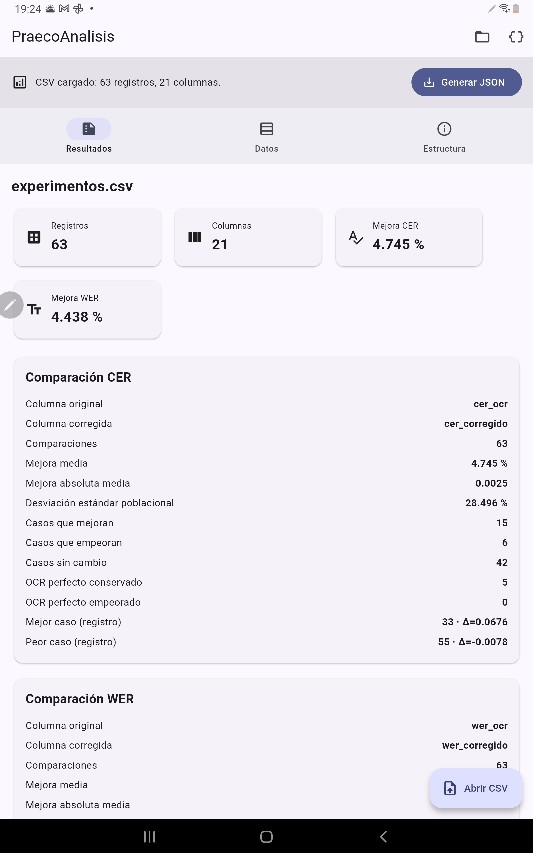
\includegraphics[
		width=\textwidth,
		height=0.39\textheight,
		keepaspectratio
		]{imagenes/16972.jpg}
		\caption{Resumen general y comparación de las métricas CER y WER.}
		\label{fig:praeco-analisis-1}
	\end{subfigure}
	\hfill
	\begin{subfigure}[t]{0.46\textwidth}
		\centering
		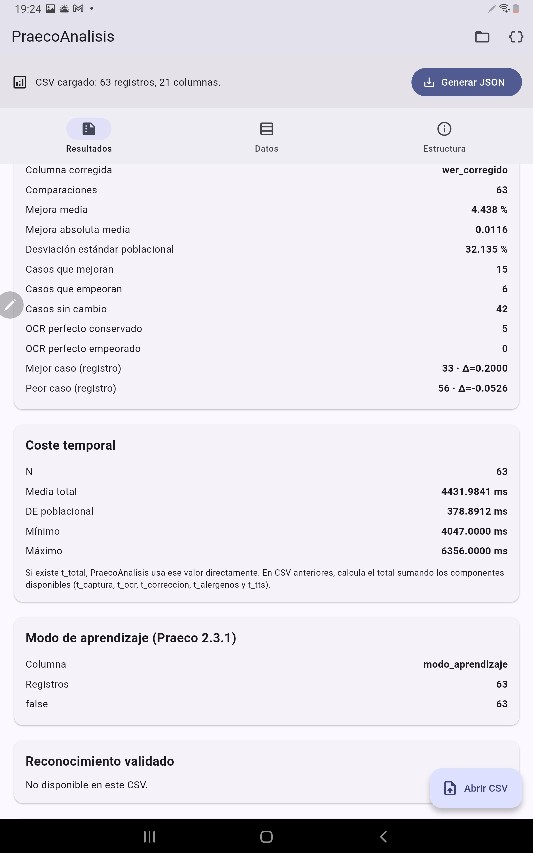
\includegraphics[
		width=\textwidth,
		height=0.39\textheight,
		keepaspectratio
		]{imagenes/16973.jpg}
		\caption{Evaluación del corrector y análisis del coste temporal.}
		\label{fig:praeco-analisis-2}
	\end{subfigure}
	
	\vspace{0.5cm}
	
	% =====================================================
	% SEGUNDA FILA
	% =====================================================
	
	\begin{subfigure}[t]{0.46\textwidth}
		\centering
		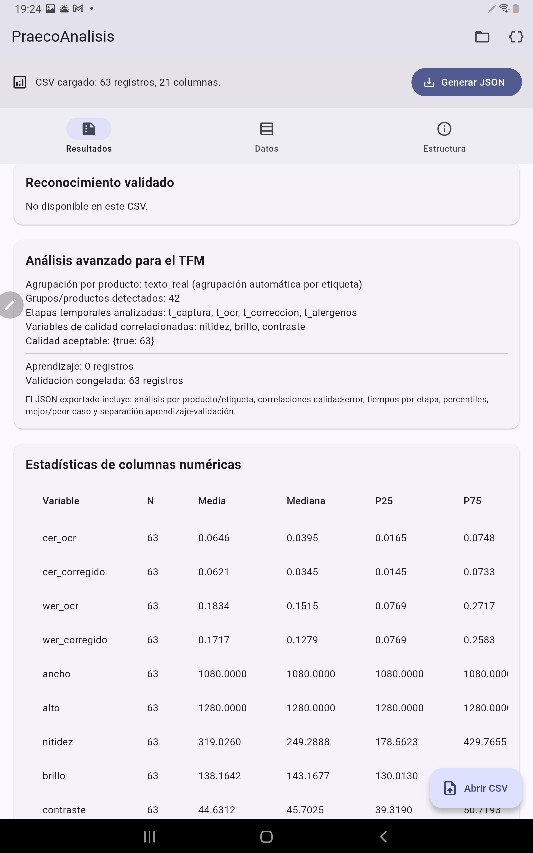
\includegraphics[
		width=\textwidth,
		height=0.39\textheight,
		keepaspectratio
		]{imagenes/16974.jpg}
		\caption{Análisis avanzado y estadísticos de las variables registradas.}
		\label{fig:praeco-analisis-3}
	\end{subfigure}
	\hfill
	\begin{subfigure}[t]{0.46\textwidth}
		\centering
		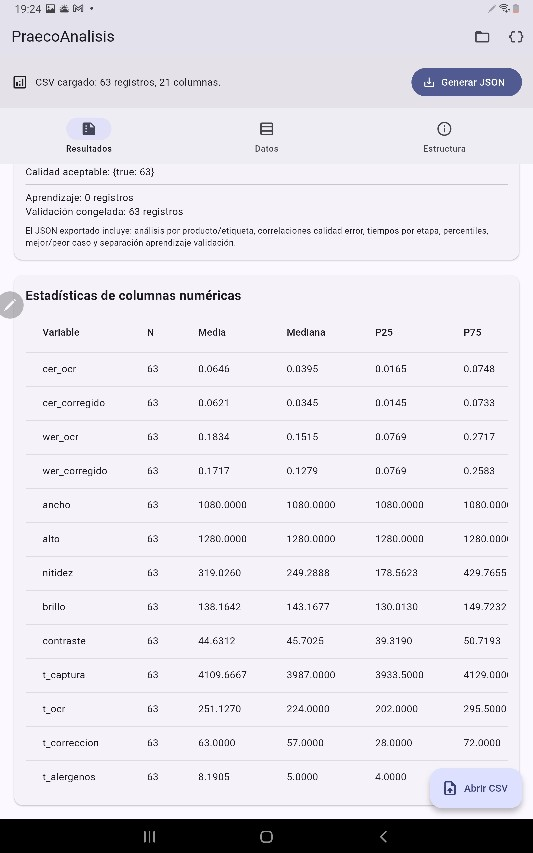
\includegraphics[
		width=\textwidth,
		height=0.39\textheight,
		keepaspectratio
		]{imagenes/16975.jpg}
		\caption{Estadísticos de calidad y tiempos de procesamiento.}
		\label{fig:praeco-analisis-4}
	\end{subfigure}
	
	\caption{Pantallas de ejemplo de Praeco Análisis.}
	
	\label{fig:praeco-analisis-pantallas}
\end{figure}

\newpage

% ------------------------------------------------
\section{Discusión de los resultados}
% ------------------------------------------------

Los resultados obtenidos a lo largo del desarrollo de Praeco muestran que la evaluación del corrector no puede reducirse únicamente a comprobar si los valores medios de CER o WER disminuyen. Aunque estas métricas permiten cuantificar de forma objetiva la precisión del reconocimiento, resulta igualmente necesario estudiar el comportamiento del corrector registro a registro, su estabilidad y, especialmente, su capacidad para conservar aquellas palabras que el OCR ya ha reconocido correctamente.

Debe tenerse en cuenta, además, que el fichero \texttt{experimentos.csv} se ha construido de forma incremental durante el desarrollo del proyecto. Los registros almacenados corresponden a distintas fases de análisis, ajuste y mejora de la aplicación. Paralelamente, durante las etapas en las que el aprendizaje se encontraba habilitado, se fue enriqueciendo el fichero \texttt{diccionario\_adaptativo.json} con vocabulario validado a partir de los experimentos realizados. Por tanto, el conjunto completo de registros refleja también la evolución del sistema y no debe interpretarse como un único ensayo realizado con una versión estática de Praeco.

Las primeras versiones del corrector mostraron que una estrategia excesivamente permisiva podía solucionar determinados errores del OCR y, simultáneamente, introducir sustituciones incorrectas sobre palabras que originalmente eran válidas. Esta situación explica que algunos experimentos presentasen mejoras locales mientras que las métricas globales permanecían prácticamente constantes o incluso empeoraban. Estos resultados fueron especialmente útiles durante el desarrollo, ya que permitieron identificar la necesidad de aumentar el carácter conservador del corrector.

Como consecuencia de este análisis se incorporaron progresivamente reglas de protección, criterios de confianza, control de conflictos y vocabulario adaptativo. El objetivo dejó de ser corregir el mayor número posible de palabras para pasar a modificar únicamente aquellas para las que existe evidencia suficiente de que se ha producido un error de reconocimiento.

El \texttt{diccionario\_adaptativo.json} constituye un elemento relevante en esta evolución. Su contenido representa vocabulario validado durante las fases de desarrollo y permite que términos encontrados previamente puedan ser reconocidos posteriormente como palabras válidas. De este modo se evita que el corrector sustituya innecesariamente términos correctos y se facilita la obtención de una salida \texttt{ocr\_corregido} más precisa. Conviene señalar que este mecanismo no modifica directamente el funcionamiento interno de Google ML Kit ni el texto OCR bruto, sino que actúa en la etapa posterior de corrección desarrollada específicamente en Praeco.

El análisis del conjunto formado por 63 registros, realizado con \texttt{modo\_aprendizaje = false}, permite evaluar el comportamiento del sistema utilizando los recursos lingüísticos previamente adquiridos pero manteniéndolos congelados durante la validación. En este conjunto, el CER medio pasa de 0.0646 para el OCR original a 0.0621 después de la corrección, mientras que el WER medio disminuye de 0.1834 a 0.1717. Praeco Análisis obtiene una mejora media del CER del 4.745\,\% y del WER del 4.438\,\%.

Sin embargo, esta mejora global no significa que todos los registros mejoren individualmente. En la comparación del CER, 15 registros mejoran, 6 empeoran y 42 permanecen sin cambios. Además, se conservan los cinco casos en los que el OCR era inicialmente perfecto, sin que el corrector introduzca errores en ellos. Estos resultados son coherentes con el criterio conservador adoptado: una proporción elevada de casos sin cambios no debe interpretarse necesariamente como una limitación, puesto que el objetivo es evitar modificaciones cuando no existe suficiente evidencia para realizarlas.

El análisis del WER conduce a una conclusión similar. La reducción de su valor medio indica que el corrector puede aportar una mejora global en el reconocimiento a nivel de palabra, pero siguen existiendo casos particulares en los que la corrección no produce ninguna modificación o puede introducir un empeoramiento. Por ello, el resultado agregado debe analizarse conjuntamente con el número de casos que mejoran, empeoran o permanecen inalterados.

El aprendizaje adaptativo tampoco debe interpretarse como un mecanismo de traducción o normalización automática al castellano. Su finalidad consiste en incorporar conocimiento validado del dominio. Las etiquetas comerciales pueden contener nombres propios, marcas, términos técnicos y vocabulario perteneciente a otros idiomas. Cuando estos términos aparecen realmente en el \textit{ground truth}, deben considerarse palabras válidas y conservarse. Un término extranjero correctamente reconocido no constituye por sí mismo un error de OCR.

Otro aspecto relevante es el coste temporal introducido por las diferentes etapas. Para el conjunto de 63 registros, Praeco Análisis obtiene un tiempo medio total de aproximadamente 4432~ms. La mayor parte corresponde al proceso de captura y selección de la imagen, con aproximadamente 4110~ms de media. El reconocimiento OCR requiere alrededor de 251~ms, mientras que la corrección presenta un tiempo medio próximo a 63~ms y la detección de alérgenos aproximadamente 8~ms. Estos resultados muestran que las etapas específicas de corrección y detección añadidas por Praeco representan una fracción reducida del tiempo total de procesamiento.

Desde el punto de vista funcional, este comportamiento resulta especialmente importante debido al objetivo asistencial de la aplicación. El texto corregido se utiliza posteriormente para la detección de términos asociados a alérgenos y para su reproducción mediante síntesis de voz. Una corrección incorrecta puede, por tanto, propagarse hacia las etapas posteriores. Esta circunstancia justifica que el sistema priorice la conservación de palabras válidas frente a una estrategia más agresiva orientada únicamente a maximizar el número de sustituciones.

Finalmente, la separación del sistema en Praeco Desarrollo, Praeco Usuario y Praeco Análisis ha permitido diferenciar claramente tres funciones. Praeco Desarrollo proporciona los mecanismos de experimentación, aprendizaje y generación de resultados; Praeco Usuario utiliza los recursos lingüísticos obtenidos sin necesidad de \textit{ground truth} ni aprendizaje durante el uso normal; y Praeco Análisis permite procesar los resultados experimentales, calcular estadísticos, comparar CER y WER, analizar el coste temporal y estudiar el comportamiento del corrector.

% ------------------------------------------------
\section{Ensayos exploratorios de captura rápida e iluminación asistida}

Después de la validación principal de 63 registros se desarrolló una versión de captura optimizada con una sola fotografía, control de linterna y mejora condicional. Los resultados de esta etapa constituyen \textbf{pruebas exploratorias posteriores}, no una ampliación de la muestra de validación del corrector ni un ensayo controlado de CLAHE.

En dos registros de la prueba con umbral de linterna 150 se obtuvieron los valores de la Tabla~\ref{tab:captura-rapida}. Las imágenes fueron aceptadas y el OCR corregido alcanzó CER y WER nulos en ambos casos.

\begin{table}[htbp]
\centering\small
\caption{Dos ensayos exploratorios de captura rápida con umbral de iluminación 150.}
\label{tab:captura-rapida}
\begin{tabular}{lrr}
\hline
\textbf{Indicador} & \textbf{Mejillones Galica} & \textbf{Don Simón}\\ \hline
Brillo medio & 132,93 & 163,73\\
Nitidez & 511,41 & 402,35\\
Contraste & 44,46 & 37,52\\
Tiempo de captura (ms) & 1842 & 1530\\
Tiempo OCR (ms) & 194 & 114\\
CER antes de corrección & 0,0172 & 0,0167\\
CER después de corrección & 0 & 0\\
WER después de corrección & 0 & 0\\ \hline
\end{tabular}
\end{table}

El tiempo medio de captura de estas dos observaciones fue 1686~ms, frente a los aproximadamente 4110~ms de captura media de la validación anterior. La diferencia descriptiva es de 2424~ms (aproximadamente un 59\,\%), pero \textbf{no puede interpretarse como una mejora causal demostrada}, porque los conjuntos de imágenes y las condiciones experimentales no son equivalentes y el alcance de los temporizadores debe comprobarse. El brillo de 132,93 corresponde a la imagen registrada y no prueba por sí solo el estado de la linterna durante la vista previa.

En ambos registros el OCR se realizó sobre la imagen original; por ello, \textbf{no se atribuye a CLAHE la reducción de CER o WER}. Para demostrar la aportación de esta técnica será necesario comparar, sobre las mismas capturas, OCR original frente a OCR con CLAHE, con el corrector y los recursos de aprendizaje congelados. También se requiere registrar el brillo previo, el estado de la linterna y el tiempo de estabilización para caracterizar el control de iluminación.

\section{Conclusiones del análisis experimental}
% ------------------------------------------------

Los resultados obtenidos durante las diferentes etapas de desarrollo y validación permiten extraer las siguientes conclusiones:

\begin{itemize}
	
	\item Las métricas CER y WER permiten cuantificar objetivamente tanto los errores producidos por el OCR como el efecto posterior del corrector desarrollado para Praeco.
	
	\item Las primeras versiones demostraron que una estrategia de corrección excesivamente permisiva puede introducir falsos positivos y empeorar palabras que originalmente habían sido reconocidas correctamente.
	
	\item La incorporación de reglas de protección, criterios de confianza y mecanismos de validación ha permitido evolucionar hacia una estrategia de corrección más conservadora.
	
	\item El aprendizaje adaptativo permite construir progresivamente un vocabulario específico a partir de información validada durante la fase de desarrollo. Este conocimiento queda almacenado principalmente en \texttt{diccionario\_adaptativo.json} y puede ser reutilizado posteriormente por el corrector.
	
	\item El fichero \texttt{experimentos.csv} refleja la evolución experimental de Praeco, puesto que se ha ido ampliando durante las diferentes etapas de análisis y mejora de la aplicación. Por esta razón, sus registros no deben interpretarse necesariamente como resultados obtenidos con una única versión estática del sistema.
	
	\item Los experimentos realizados con \texttt{modo\_aprendizaje = true} pertenecen a la fase de adquisición de conocimiento y no deben confundirse con una validación independiente del sistema.
	
	\item La utilización de \texttt{modo\_aprendizaje = false} permite congelar los recursos adquiridos y evaluar el comportamiento del corrector sin que los propios datos de validación modifiquen simultáneamente el sistema.
	
	\item En el conjunto analizado de 63 registros con aprendizaje desactivado se obtiene una mejora global de las métricas. El CER medio disminuye de 0.0646 a 0.0621 y el WER medio de 0.1834 a 0.1717, correspondientes a mejoras medias calculadas por Praeco Análisis del 4.745\,\% y del 4.438\,\%, respectivamente.
	
	\item La mejora global no implica una mejora individual en todos los casos. Para CER, 15 registros mejoran, 6 empeoran y 42 permanecen sin cambios. Los cinco casos con OCR inicialmente perfecto se conservan sin introducir errores, lo que constituye un indicador relevante del carácter conservador del corrector.
	
	\item La auditoría manual del \textit{ground truth} resulta imprescindible para que los valores obtenidos de CER y WER representen correctamente el error real del sistema.
	
	\item El vocabulario multilingüe, los nombres propios, las marcas y otros términos presentes legítimamente en las etiquetas deben conservarse y no considerarse automáticamente errores. El aprendizaje adaptativo no constituye un mecanismo de traducción.
	
	\item El análisis temporal muestra que el coste añadido específicamente por la corrección y la detección de alérgenos es reducido respecto al tiempo total de procesamiento. La mayor parte del tiempo corresponde al proceso de adquisición y selección de la imagen.
	
	\item La separación entre Praeco Desarrollo, Praeco Usuario y Praeco Análisis permite distinguir claramente las fases de experimentación y aprendizaje, utilización del asistente y evaluación de los resultados.
	
\end{itemize}

En conjunto, los resultados permiten concluir que el corrector de Praeco produce una mejora global moderada de las métricas CER y WER en el conjunto de validación analizado, aunque dicha mejora no se produce de manera uniforme en todos los registros. Este comportamiento confirma la conveniencia de utilizar una estrategia conservadora, en la que una palabra únicamente se modifica cuando existe evidencia suficiente para realizar la corrección.

La evolución del \texttt{diccionario\_adaptativo.json} permite incorporar conocimiento validado durante el desarrollo y reutilizarlo posteriormente sin modificar los recursos durante la fase de validación. La combinación de aprendizaje previo, congelación de los recursos y evaluación posterior proporciona una metodología más rigurosa que la utilización simultánea de aprendizaje y validación sobre los mismos datos.

Por último, el desarrollo de Praeco no se limita al reconocimiento óptico de caracteres, sino que integra adquisición y selección automática de imágenes, OCR, corrección léxica, aprendizaje adaptativo, detección de términos asociados a alérgenos, síntesis de voz y herramientas específicas para la evaluación experimental. Los resultados obtenidos muestran que esta arquitectura puede ejecutarse en un dispositivo móvil con un coste adicional reducido para las etapas de corrección y detección, manteniendo como criterio fundamental la conservación del texto correctamente reconocido.

